\documentclass{article}

  % packages
    % basic stuff for rendering math
    \usepackage[letterpaper, top=1in, bottom=1in, left=1in, right=1in]{geometry}
    \usepackage[utf8]{inputenc}
    \usepackage[english]{babel}
    \usepackage{amsmath} 
    \usepackage{amssymb}

    % extra math symbols and utilities
    \usepackage{mathtools}        % for extra stuff like \coloneqq
    \usepackage{mathrsfs}         % for extra stuff like \mathsrc{}
    \usepackage{centernot}        % for the centernot arrow 
    \usepackage{bm}               % for better boldsymbol/mathbf 
    \usepackage{enumitem}         % better control over enumerate, itemize
    \usepackage{hyperref}         % for hypertext linking
    \usepackage{xr-hyper}
    \usepackage{fancyvrb}          % for better verbatim environments
    \usepackage{newverbs}         % for texttt{}
    \usepackage{xcolor}           % for colored text 
    \usepackage{listings}         % to include code
    \usepackage{lstautogobble}    % helper package for code
    \usepackage{parcolumns}       % for side by side columns for two column code
    

    % page layout
    \usepackage{fancyhdr}         % for headers and footers 
    \usepackage{lastpage}         % to include last page number in footer 
    \usepackage{parskip}          % for no indentation and space between paragraphs    
    \usepackage[T1]{fontenc}      % to include \textbackslash
    \usepackage{footnote}
    \usepackage{etoolbox}

    % for custom environments
    \usepackage{tcolorbox}        % for better colored boxes in custom environments
    \tcbuselibrary{breakable}     % to allow tcolorboxes to break across pages

    % figures
    \usepackage{pgfplots}
    \pgfplotsset{compat=1.18}
    \usepackage{float}            % for [H] figure placement
    \usepackage{tikz}
    \usepackage{tikz-cd}
    \usepackage{circuitikz}
    \usetikzlibrary{arrows}
    \usetikzlibrary{positioning}
    \usetikzlibrary{calc}
    \usepackage{graphicx}
    \usepackage{algorithmic}
    \usepackage{caption} 
    \usepackage{subcaption}
    \captionsetup{font=small}

    % for tabular stuff 
    \usepackage{dcolumn}

    \usepackage[nottoc]{tocbibind}
    \pdfsuppresswarningpagegroup=1
    \hfuzz=5.002pt                % ignore overfull hbox badness warnings below this limit

  % New and replaced operators
    \DeclareMathOperator{\Tr}{Tr}
    \DeclareMathOperator{\Sym}{Sym}
    \DeclareMathOperator{\Span}{span}
    \DeclareMathOperator{\std}{std}
    \DeclareMathOperator{\Cov}{Cov}
    \DeclareMathOperator{\Var}{Var}
    \DeclareMathOperator{\Corr}{Corr}
    \DeclareMathOperator{\pos}{pos}
    \DeclareMathOperator*{\argmin}{\arg\!\min}
    \DeclareMathOperator*{\argmax}{\arg\!\max}
    \newcommand{\ket}[1]{\ensuremath{\left|#1\right\rangle}}
    \newcommand{\bra}[1]{\ensuremath{\left\langle#1\right|}}
    \newcommand{\braket}[2]{\langle #1 | #2 \rangle}
    \newcommand{\qed}{\hfill$\blacksquare$}     % I like QED squares to be black

  % Custom Environments
    \newtcolorbox[auto counter, number within=section]{question}[1][]
    {
      colframe = orange!25,
      colback  = orange!10,
      coltitle = orange!20!black,  
      breakable, 
      title = \textbf{Question \thetcbcounter ~(#1)}
    }

    \newtcolorbox[auto counter, number within=section]{exercise}[1][]
    {
      colframe = teal!25,
      colback  = teal!10,
      coltitle = teal!20!black,  
      breakable, 
      title = \textbf{Exercise \thetcbcounter ~(#1)}
    }
    \newtcolorbox[auto counter, number within=section]{solution}[1][]
    {
      colframe = violet!25,
      colback  = violet!10,
      coltitle = violet!20!black,  
      breakable, 
      title = \textbf{Solution \thetcbcounter}
    }
    \newtcolorbox[auto counter, number within=section]{lemma}[1][]
    {
      colframe = red!25,
      colback  = red!10,
      coltitle = red!20!black,  
      breakable, 
      title = \textbf{Lemma \thetcbcounter ~(#1)}
    }
    \newtcolorbox[auto counter, number within=section]{theorem}[1][]
    {
      colframe = red!25,
      colback  = red!10,
      coltitle = red!20!black,  
      breakable, 
      title = \textbf{Theorem \thetcbcounter ~(#1)}
    } 
    \newtcolorbox[auto counter, number within=section]{proposition}[1][]
    {
      colframe = red!25,
      colback  = red!10,
      coltitle = red!20!black,  
      breakable, 
      title = \textbf{Proposition \thetcbcounter ~(#1)}
    } 
    \newtcolorbox[auto counter, number within=section]{corollary}[1][]
    {
      colframe = red!25,
      colback  = red!10,
      coltitle = red!20!black,  
      breakable, 
      title = \textbf{Corollary \thetcbcounter ~(#1)}
    } 
    \newtcolorbox[auto counter, number within=section]{proof}[1][]
    {
      colframe = orange!25,
      colback  = orange!10,
      coltitle = orange!20!black,  
      breakable, 
      title = \textbf{Proof. }
    } 
    \newtcolorbox[auto counter, number within=section]{definition}[1][]
    {
      colframe = yellow!25,
      colback  = yellow!10,
      coltitle = yellow!20!black,  
      breakable, 
      title = \textbf{Definition \thetcbcounter ~(#1)}
    } 
    \newtcolorbox[auto counter, number within=section]{example}[1][]
    {
      colframe = blue!25,
      colback  = blue!10,
      coltitle = blue!20!black,  
      breakable, 
      title = \textbf{Example \thetcbcounter ~(#1)}
    } 
    \newtcolorbox[auto counter, number within=section]{code}[1][]
    {
      colframe = green!25,
      colback  = green!10,
      coltitle = green!20!black,  
      breakable, 
      title = \textbf{Code \thetcbcounter ~(#1)}
    } 
    \newtcolorbox[auto counter, number within=section]{algo}[1][]
    {
      colframe = green!25,
      colback  = green!10,
      coltitle = green!20!black,  
      breakable, 
      title = \textbf{Algorithm \thetcbcounter ~(#1)}
    } 

    \definecolor{dkgreen}{rgb}{0,0.6,0}
    \definecolor{gray}{rgb}{0.5,0.5,0.5}
    \definecolor{mauve}{rgb}{0.58,0,0.82}
    \definecolor{darkblue}{rgb}{0,0,139}
    \definecolor{lightgray}{gray}{0.93}
    \renewcommand{\algorithmiccomment}[1]{\hfill$\triangleright$\textcolor{blue}{#1}}

    % default options for listings (for code)
    \lstset{
      autogobble,
      frame=ltbr,
      language=Python,
      aboveskip=3mm,
      belowskip=3mm,
      showstringspaces=false,
      columns=fullflexible,
      keepspaces=true,
      basicstyle={\small\ttfamily},
      numbers=left,
      firstnumber=1,                        % start line number at 1
      numberstyle=\tiny\color{gray},
      keywordstyle=\color{blue},
      commentstyle=\color{dkgreen},
      stringstyle=\color{mauve},
      backgroundcolor=\color{lightgray}, 
      breaklines=true,                      % break lines
      breakatwhitespace=true,
      tabsize=3, 
      xleftmargin=2em, 
      framexleftmargin=1.5em, 
      stepnumber=1
    }

  % Page style
    \pagestyle{fancy}
    \fancyhead[L]{Clustering}
    \fancyhead[C]{Muchang Bahng}
    \fancyhead[R]{Spring 2025} 
    \fancyfoot[C]{\thepage / \pageref{LastPage}}
    \renewcommand{\footrulewidth}{0.4pt}          % the footer line should be 0.4pt wide
    \renewcommand{\thispagestyle}[1]{}  % needed to include headers in title page

  % external documents 
  %  \externaldocument[place-]{../Machine_Learning/paper}[../Machine_Learning/paper.pdf] 

\begin{document}

\title{Clustering and Density Estimation}
\author{Muchang Bahng}
\date{Spring 2025}

\maketitle
\tableofcontents
\pagebreak

This covers computability theory, complexity theory, and automata theory. 
Alphabet. Boolean logic


\section{K Means Clustering} 

  We will start off with conceptually the simplest form of clustering, although not the earliest developed. K-means was published at 1967 in \cite{1967macqueen}, but has been discovered in the 1950s. The general idea is that given an integer $K$, we want to find $K$ \textit{centroids} that provide a good approximation of where the clusters are in the data. We can quantify what a good approximation is by taking the distance from a sample to its closest cluster centroid.

  \begin{definition}[K Means Clustering]
    A \textbf{K-means clustering} model is an parameteric unsupervised model with parameters $\{\mu_1, \ldots, \mu_K\}$ representing clusters that each sample belongs to. The cluster that sample $x$ belongs to is 
    \begin{equation}
      \mathrm{cluster}(x) = \argmin_{\mu_k} d(x, \mu_k)
    \end{equation}
    Usually, we let $d$ be the $L^2$ metric in Euclidean space. 
  \end{definition}

  \begin{theorem}[Risk]
    The expected risk of $K$-means is 
    \begin{equation}
      R(\mu_1, \ldots, \mu_K) = \mathbb{E}_x \left[ \min_{k \in [K]} \| x - \mu_k \|^2 \right] = \int \min_{k \in [K]} \| x - \mu_k \|^2 \,dx
    \end{equation} 
    and our empirical risk for a dataset $\mathcal{D} = \{x^{(i)}\}_{i=1}^n$ is therefore 
    \begin{equation}
      \hat{R}(\mu_1, \ldots, \mu_K) = \frac{1}{n} \sum_{i=1}^n \min_{k \in [K]} \| x^{(i)} - \mu_k \|^2
    \end{equation} 
  \end{theorem} 

\subsection{NP-Hardness}

  So we have reduced this model into an optimization problem of the appropriate risk. Let's try and analyze how hard this is. 

  \begin{theorem}
    For a fixed dimension $d$ and number of clusters $K$, we can minimize the empirical risk in $O(n^{dk + 1})$. 
  \end{theorem} 

  \begin{theorem}
    For any fixed $d$ (even $d = 2$), minimizing the empirical risk over all $K$ is NP-hard. 
  \end{theorem}

  Therefore, we must rely on approximate algorithms. 

\subsection{Lloyd's Algorithm}

  Great, we have an almost-everywhere differentiable function, which can be solved with gradient methods like SGD or coordinate descent. The problem is that this is not necessarily convex. 

  \begin{theorem}[Convergence of Coordinate Descent]
    
  \end{theorem}
  
  Now that convergence is guaranteed, constructing the algorithm is straightforward. In fact, it is precisely coordinate descent!  

  \begin{algo}[Lloyd's Algorithm]
    The algorithm intuitively initializes the centroids randomly, and then moves them to the center of each cluster through the two stage process: 
    \begin{enumerate}
      \item Assigning each training sample $x^{(i)}$ to the closest cluster centroid $\mu_k$. 
      \item Move each training cluster centroid $\mu_k$ to the mean of the points assigned to it. 
    \end{enumerate}
    \begin{algorithm}[H]
    \caption{K-Means Clustering}
    \label{alg:kmeans}
    \begin{algorithmic}[1]
      \Procedure{KMeans}{$\mathbf{X}, K$}
          
      \Require{Dataset $\mathbf{X} = \{x^{(1)}, x^{(2)}, \ldots, x^{(n)}\}$ where $x^{(i)} \in \mathbb{R}^d$, number of clusters $K$}
      \Ensure{Cluster centroids $\mu_1, \mu_2, \ldots, \mu_K$ and cluster assignments $c^{(1)}, c^{(2)}, \ldots, c^{(n)}$}
      
      % Initialization
      \State Initialize cluster centroids $\mu_1, \mu_2, \ldots, \mu_K \in \mathbb{R}^d$ randomly
      
      % Main loop
      \Repeat
        % Assignment step
        \For{$i \gets 1$ to $n$}
          \State $c^{(i)} \gets \arg\min_j ||x^{(i)} - \mu_j||^2$
        \EndFor
        
        % Update step
        \For{$j \gets 1$ to $K$}
          \State $\mu_j \gets \frac{\sum_{i=1}^n \mathbf{1}\{c^{(i)} = k\} x^{(i)}}{\sum_{i=1}^n \mathbf{1}\{c^{(i)} = k\}}$
        \EndFor
      \Until{convergence}
      
      \State \Return $\mu_1, \mu_2, \ldots, \mu_K, c^{(1)}, c^{(2)}, \ldots, c^{(n)}$
      \EndProcedure
    \end{algorithmic}
    \end{algorithm}
  \end{algo} 

  \begin{example}[K-Means Walkthrough]
    Let us walk through how the centroids evolve visually on a toy dataset. 

    \begin{figure}[H]
      \centering
      \begin{subfigure}[b]{0.48\textwidth}
        \centering
        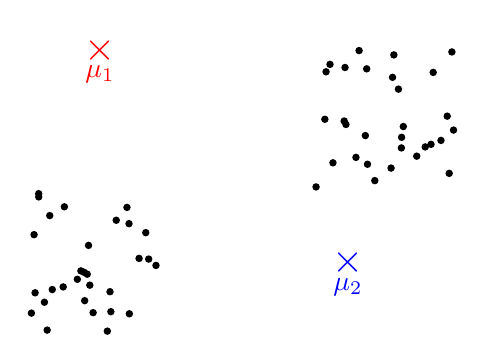
\begin{tikzpicture}[scale=0.9]
          \pgfmathsetseed{42}
          \foreach \i in {1,...,30} { 
            \pgfmathsetmacro{\x}{-2 + 2*rnd }
            \pgfmathsetmacro{\y}{-1 + 2*rnd}
            \fill[black] (\x,\y) circle (1.5pt);
          }

          \foreach \i in {1,...,30} {
            \pgfmathsetmacro{\x}{2 + 2*rnd}
            \pgfmathsetmacro{\y}{1 + 2*rnd}
            \fill[black] (\x,\y) circle (1.5pt);
          }

          % Left centroid
          \node[red, font=\Large] at (-1,3) {$\times$};
          \node[red, below=2pt] at (-1,3) {$\mu_1$};

          % Right centroid
          \node[blue, font=\Large] at (2.5,0) {$\times$};
          \node[blue, below=2pt] at (2.5,0) {$\mu_2$};
        \end{tikzpicture}
        \caption{We initialize the centroids $\mu_1, \mu_2$ randomly.}
      \end{subfigure}
      \hfill 
      \begin{subfigure}[b]{0.48\textwidth}
        \centering
        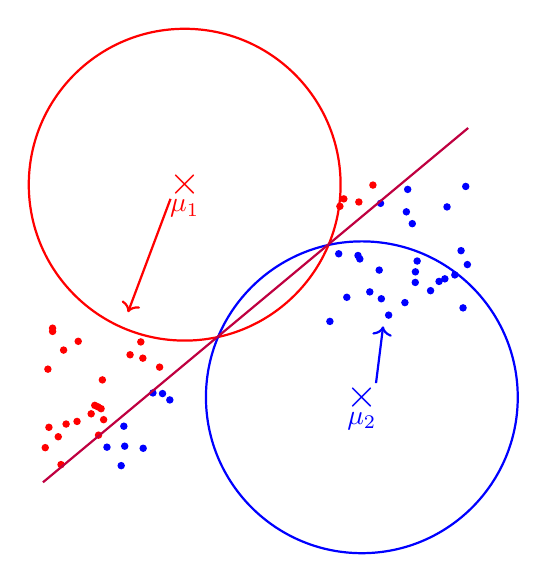
\begin{tikzpicture}[scale=0.9]
          \pgfmathsetseed{42}
          \foreach \i in {1,...,30} { 
            \pgfmathsetmacro{\x}{-2 + 2*rnd }
            \pgfmathsetmacro{\y}{-1 + 2*rnd}
            % Calculate if point is above or below the purple line y = 0.833x + 0.467
            \pgfmathsetmacro{\liney}{0.833*\x + 0.467}
            \pgfmathsetmacro{\isabove}{\y > \liney ? 1 : 0}
            \ifnum\isabove=1
              \fill[red] (\x,\y) circle (1.5pt);
            \else
              \fill[blue] (\x,\y) circle (1.5pt);
            \fi
          }
          \foreach \i in {1,...,30} {
            \pgfmathsetmacro{\x}{2 + 2*rnd}
            \pgfmathsetmacro{\y}{1 + 2*rnd}
            % Calculate if point is above or below the purple line y = 0.833x + 0.467
            \pgfmathsetmacro{\liney}{0.833*\x + 0.467}
            \pgfmathsetmacro{\isabove}{\y > \liney ? 1 : 0}
            \ifnum\isabove=1
              \fill[red] (\x,\y) circle (1.5pt);
            \else
              \fill[blue] (\x,\y) circle (1.5pt);
            \fi
          }
          % Left centroid
          \node[red, font=\Large] at (0,3) {$\times$};
          \node[red, below=2pt] at (0,3) {$\mu_1$};
          \draw[red, thick] (0,3) circle (2.2cm);  % Red circle around μ₁
          
          % Right centroid
          \node[blue, font=\Large] at (2.5,0) {$\times$};
          \node[blue, below=2pt] at (2.5,0) {$\mu_2$};
          \draw[blue, thick] (2.5,0) circle (2.2cm);  % Blue circle around μ₂ 
          \draw[purple, thick] (-2, -1.2) -- (4, 3.8);
          \draw[red, thick, ->] (-0.2, 2.8) -- (-0.8, 1.2);
          \draw[blue, thick, ->] (2.7, 0.2) -- (2.8, 1);
        \end{tikzpicture}
        \caption{We classify all points that are in clusters $1$ and $2$. }
      \end{subfigure}

      \begin{subfigure}[b]{0.48\textwidth}
        \centering
        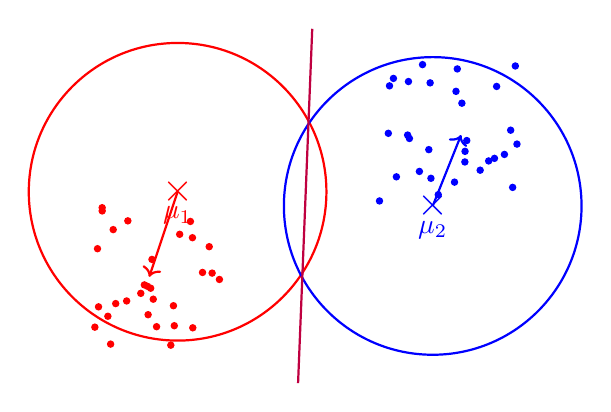
\begin{tikzpicture}[scale=0.9]
          \pgfmathsetseed{42}
          \foreach \i in {1,...,30} { 
            \pgfmathsetmacro{\x}{-2 + 2*rnd }
            \pgfmathsetmacro{\y}{-1 + 2*rnd}
              \fill[red] (\x,\y) circle (1.5pt);
          }
          \foreach \i in {1,...,30} {
            \pgfmathsetmacro{\x}{2 + 2*rnd}
            \pgfmathsetmacro{\y}{1 + 2*rnd} 
            \fill[blue] (\x,\y) circle (1.5pt);
          }
          % Left centroid (moved to arrow head)
          \node[red, font=\Large] at (-0.8,1.2) {$\times$};
          \node[red, below=2pt] at (-0.8,1.2) {$\mu_1$};
          \draw[red, thick] (-0.8,1.2) circle (2.1cm);  % Red circle around μ₁
          
          % Right centroid (moved to arrow head)
          \node[blue, font=\Large] at (2.8,1) {$\times$};
          \node[blue, below=2pt] at (2.8,1) {$\mu_2$};
          \draw[blue, thick] (2.8,1) circle (2.1cm);  % Blue circle around μ₂ 
          
          % New decision boundary line (perpendicular bisector of the line connecting the centroids)
          \draw[purple, thick] (1.1, 3.5) -- (0.9, -1.5);
          \draw[red, thick, ->] (-0.8, 1.2) -- (-1.2, -0);
          \draw[blue, thick, ->] (2.8, 1) -- (3.2, 2);
        \end{tikzpicture}
        \caption{We update the centroids and classify again.}
      \end{subfigure}
      \hfill 
      \begin{subfigure}[b]{0.48\textwidth}
        \centering
        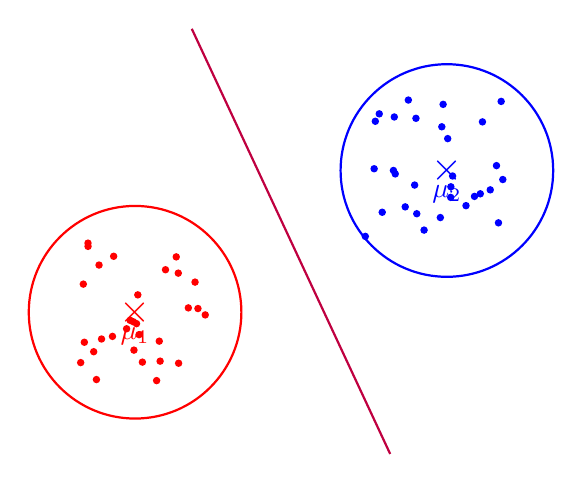
\begin{tikzpicture}[scale=0.9]
          \pgfmathsetseed{42}
          \foreach \i in {1,...,30} { 
            \pgfmathsetmacro{\x}{-2 + 2*rnd }
            \pgfmathsetmacro{\y}{-1 + 2*rnd}
              \fill[red] (\x,\y) circle (1.5pt);
          }
          \foreach \i in {1,...,30} {
            \pgfmathsetmacro{\x}{2 + 2*rnd}
            \pgfmathsetmacro{\y}{1 + 2*rnd} 
            \fill[blue] (\x,\y) circle (1.5pt);
          }
          % Left centroid (moved to arrow head)
          \node[red, font=\Large] at (-1.2, -0) {$\times$};
          \node[red, below=2pt] at (-1.2, -0) {$\mu_1$};
          \draw[red, thick] (-1.2, -0) circle (1.5cm);  % Red circle around μ₁
          
          % Right centroid (moved to arrow head)
          \node[blue, font=\Large] at (3.2, 2) {$\times$};
          \node[blue, below=2pt] at (3.2, 2) {$\mu_2$};
          \draw[blue, thick] (3.2, 2) circle (1.5cm);  % Blue circle around μ₂ 
          
          % New decision boundary line (perpendicular bisector of the line connecting the centroids)
          \draw[purple, thick] (-0.4, 4) -- (2.4, -2);
        \end{tikzpicture}
        \caption{We have convergence.}
      \end{subfigure}
      \caption{A walkthrough for $K$-means clustering for $K = 2$ in $\mathbb{R}^2$.}
      \label{fig:kmeans}
    \end{figure}
  \end{example}

\subsection{Concentration Bounds}

  We can bound the supremum of the expected and exmpirical risk either through the VC dimension or directly with the Rademacher complexity. They both give different bounds, which have advantages and disadvantages. 

  \begin{theorem}
    Let us work over a compact domain. Given that $C^\ast$ is the true risk minimizer and $\hat{C}$ is our empirical risk minimizer, 
    \begin{equation}
      C^\ast = \argmin_{\mu_1, \ldots, \mu_K} R(C), \qquad \hat{C} = \argmin_{\mu_1, \ldots, \mu_K} \hat{R}(C) 
    \end{equation}
    we have 
    \begin{equation}
      \mathbb{E} \left[ | R(C^\ast) - R(\hat{C}) \right] \leq \sqrt{\frac{K (d+1) \log{n}}{n}}
    \end{equation}
  \end{theorem}
  \begin{proof}
    This is proved using VC dimension. 
  \end{proof}

  Let's parse this. So the more clusters you're trying to find---the bigger the $K$---the worse the bound is. More disturbing is the dimension $d$. If $d$ is big, then this is not a very good bound. 

  \begin{theorem}[2008 Gao, Deroit?, Lugacy?]
    Let us work over a compact domain. Given that $C^\ast$ is the true risk minimizer and $\hat{C}$ is our empirical risk minimizer, 
    \begin{equation}
      C^\ast = \argmin_{\mu_1, \ldots, \mu_K} R(C), \qquad \hat{C} = \argmin_{\mu_1, \ldots, \mu_K} \hat{R}(C) 
    \end{equation}
    we have 
    \begin{equation}
      \mathbb{E} \left[ | R(C^\ast) - R(\hat{C}) \right] \leq \frac{K}{n}
    \end{equation}
  \end{theorem}
  \begin{proof}
    This is proved directly using Rademacher complexity. 
  \end{proof}

  The advantage of this is that this bound is dimensionless. This is even true in infinite dimensional Hilbert spaces, which is useful when clustering functions. 

  Now just because the risks are close it does not mean that the clusters are close. You can have two sets of clusters $\{\mu_k\}, \{\mu_k^\prime\}$ that have similar risk but they can be far apart from each other. To control this we need extra assumptions. 

\subsection{Choosing Number of Clusters K}

  Note that the performance of K means really depends on a good choice of $K$. Think about what would have happened if we set $K = 5$ in the walkthrough above. Let's study the impact of changing $K$ a bit more. 

  \begin{theorem}[Expected Risk Decreases as K Increases]
    If $K < K^\prime$, then 
    \begin{equation}
      R(\mu_1, \ldots, \mu_K) \leq R(\mu_1, \ldots, \mu_{K^\prime})
    \end{equation}
  \end{theorem}
  \begin{proof}
    
  \end{proof}




\section{Multi-Dimensional Scaling}

  Again, we want to reduce our dimension, but the goal is slightly different from PCA. 

  \begin{definition}[Multi-Dimensional Scaling]
    Given our data $X \in \mathbb{R}^d$, we want to construct a linear map $T: \mathbb{R}^d \rightarrow \mathbb{R}^k$ such that it preserves the pairwise differences between the data points. That is, we want to minimize the following loss function 
    \begin{equation}
      \min_{T} \sum_{i \neq j} \big( d_{\mathbb{R}^k}(T(x_i), T(x_j)) - d_{\mathbb{R}^d}(x_i, x_j) \big)
    \end{equation}
    where $d_{V}$ is a distance metric in the space $V$. 
  \end{definition}

  Note that we can easily modify this formulation to preserve other structures, such as dot products, weights between distances, or different types of metrics in each space. It turns out that when the distance metric is the Euclidean L2 distance, then the solution to this linear map turns out to be PCA. This may be a more intuitive way to think about PCA, since we're trying to preserve the pairwise distances between the data points. 

  \begin{theorem}[Equivalence of Classical MDS and PCA]
    If the distance metric is the Euclidean L2 distance, then the solution to the MDS problem is equivalent to PCA. That is, 
    \begin{equation}
      T_k = \argmin_{T} \sum_{i \neq j} \big( ||T(x_i) - T(x_j)||^2 - ||x_i - x_j||^2 \big)
    \end{equation}
  \end{theorem}

  Generally, if you don't use classical MDS, then you will get a different answer than PCA and there doesn't exist a closed form solution, so you'll have to minimize this numerically. 

  \begin{example}[Non Classical MDS]
    The loss 
    \begin{equation}
      \sum_{i \neq j}  \big( ||T(x_i) - T(x_j)|| - ||x_i - x_j|| \big)^2 
    \end{equation}
    does not give the same solution as PCA. 
  \end{example}


\section{Isomap} 

  Isomap is a bit different in the way that it tries to capture more of the global structure of the data, which brings advantages and disadvantages. It is simply a modification of MDS but with geodesic distances. 

  You start off with the point cloud, but with every point, $x_i$, you find the local neighborhood $N_i$ and you make a weighted graph over the whole dataset in the high dimensional space. Then, the distance between any two arbitrary points is the shortest weighted sum of the path between them, calculated by Dijkstra's algorithm. Intuitively, this is an approximation of the geodesic distance, denoted $d_G$, between these two points on a manifold. 
  \begin{figure}[H]
    \centering 
    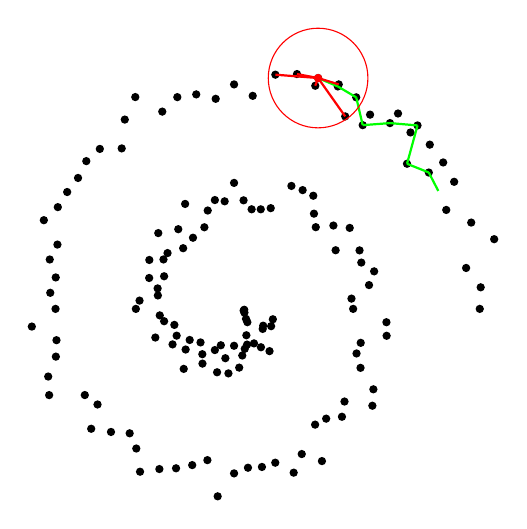
\begin{tikzpicture}
      \pgfmathsetseed{42}
      
      % Store all spiral dot coordinates first
      \foreach \t in {0,5,...,720} {
        \pgfmathsetmacro{\radius}{3 - \t/240}
        \pgfmathsetmacro{\noise}{0.5*rnd}
        \pgfmathsetmacro{\x}{(\radius + \noise) * cos(\t)}
        \pgfmathsetmacro{\y}{(\radius + \noise) * sin(\t)}
        
        \ifnum\t<720
          % Store coordinates globally
          \global\expandafter\edef\csname spiralx\t\endcsname{\x}
          \global\expandafter\edef\csname spiraly\t\endcsname{\y}
          \fill (\x, \y) circle (1.5pt);
        \fi
      }
      
      % Connect a subset of points with green lines (roughly in the top area)
      \pgfmathsetseed{42} % Reset seed to get same coordinates
      \coordinate (prev) at (0,0);
      
      \foreach \t in {30,35,40,45,50,55,60,65,70} {
        \pgfmathsetmacro{\radius}{3 - \t/240}
        \pgfmathsetmacro{\noise}{0.5*rnd}
        \pgfmathsetmacro{\x}{(\radius + \noise) * cos(\t)}
        \pgfmathsetmacro{\y}{(\radius + \noise) * sin(\t)}
        
        % Draw line from previous point (except for first point)
        \ifnum\t>30
          \fill (\x, \y) circle (1.5pt);
          \draw[green, thick] (prev) -- (\x, \y);
        \fi 
        \ifnum\t=70
          \fill[red] (\x, \y) circle (1.5pt);
          \draw[red] (\x, \y) circle (18pt);
          
          % Store red point coordinates
          \pgfmathsetmacro{\redx}{\x}
          \pgfmathsetmacro{\redy}{\y}
          \global\let\redpointx\redx
          \global\let\redpointy\redy
        \fi
        
        % Update previous coordinate
        \coordinate (prev) at (\x, \y);
      }
      
      % Draw red lines from red point to all spiral points within the circle
      \foreach \t in {0,5,...,715} {
        \pgfmathsetmacro{\px}{\csname spiralx\t\endcsname}
        \pgfmathsetmacro{\py}{\csname spiraly\t\endcsname}
        
        % Calculate distance from red point
        \pgfmathsetmacro{\dist}{sqrt((\px - \redpointx)^2 + (\py - \redpointy)^2)}
        
        % If distance is less than circle radius (18pt ≈ 0.25 inches)
        \pgfmathparse{\dist < 0.75 ? 1 : 0}
        \ifnum\pgfmathresult=1
          \draw[red, thick] (\redpointx, \redpointy) -- (\px, \py);
        \fi
      }
    \end{tikzpicture}
    \caption{The classical example is the spiral manifold. The data lies in this manifold, and the geodesic distance helps us gain an accurate distance metric within this data. } 
    \label{fig:isomap}
  \end{figure}

  \begin{definition}[Isomap] 
    Then, we simply do Isomap by minimizing 
    \begin{equation}
      \min_{T} \sum_{i \neq j} \big( d_{\mathbb{R}^k}(T(x_i), T(x_j)) - d_G(x_i, x_j) \big)
    \end{equation}
  \end{definition}

  The problem with this is that it is very sensitive to noise. For example, if we had a few points lying between the spirals, then the geodesic distance between the two spirals would be very small, and so the MDS would try to bring them closer together.  

  \begin{figure}[H]
    \centering
    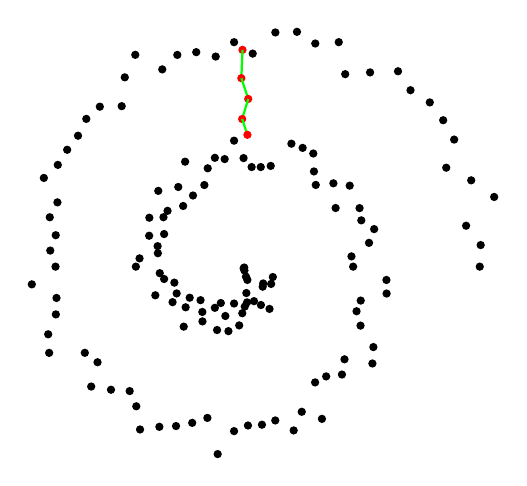
\begin{tikzpicture}
      \pgfmathsetseed{42}
      
      % Draw all spiral dots first
      \foreach \t in {0,5,...,720} {
        \pgfmathsetmacro{\radius}{3 - \t/240}
        \pgfmathsetmacro{\noise}{0.5*rnd}
        \pgfmathsetmacro{\x}{(\radius + \noise) * cos(\t)}
        \pgfmathsetmacro{\y}{(\radius + \noise) * sin(\t)}
        
        \ifnum\t<720
          \fill (\x, \y) circle (1.5pt);
        \fi
      }
      
      % Add red labeled points from top of outermost to second outermost spiral
      % Top of outermost spiral (around 90 degrees, t=90)
      \pgfmathsetseed{42}
      \foreach \step in {1,...,90} {
        \pgfmathsetmacro{\noise}{0.5*rnd}
      }
      \pgfmathsetmacro{\radiusone}{3 - 90/240}
      \pgfmathsetmacro{\noiseone}{0.5*rnd}
      \pgfmathsetmacro{\xone}{(\radiusone) * cos(90)}
      \pgfmathsetmacro{\yone}{(\radiusone) * sin(90)}
      
      % Top of second outermost spiral (around 450 degrees, t=450)
      \pgfmathsetseed{42}
      \foreach \step in {1,...,90} {
        \pgfmathsetmacro{\noise}{0.5*rnd}
      }
      \pgfmathsetmacro{\radiustwo}{3 - 450/240}
      \pgfmathsetmacro{\noisetwo}{0.5*rnd}
      \pgfmathsetmacro{\xtwo}{(\radiustwo + \noisetwo) * cos(90)}
      \pgfmathsetmacro{\ytwo}{(\radiustwo + \noisetwo) * sin(90)}
      
      % Create 7 points total (A, 5 intermediate points, B) with linear interpolation and noise
      \coordinate (prev) at (0,0);
      \foreach \i in {0,1,2,3,4} {
        \pgfmathsetmacro{\t}{\i/4}  % Parameter from 0 to 1
        \pgfmathsetmacro{\interpx}{(1-\t)*\xone + \t*\xtwo}
        \pgfmathsetmacro{\interpy}{(1-\t)*\yone + \t*\ytwo}
        
        % Add some noise to intermediate points
        \pgfmathsetmacro{\noisex}{0.2*rnd}
        \pgfmathsetmacro{\noisey}{0.2*rnd}
        \pgfmathsetmacro{\finalx}{\interpx + \noisex}
        \pgfmathsetmacro{\finaly}{\interpy + \noisey}
        
        % Draw green line from previous point (except for first point)
        \ifnum\i>0
          \draw[green, thick] (prev) -- (\finalx, \finaly);
        \fi
        
        % Draw red point
        \fill[red] (\finalx, \finaly) circle (1.5pt);
        
        % Update previous coordinate
        \coordinate (prev) at (\finalx, \finaly);
      }
    \end{tikzpicture}
    \caption{With extra noisy points (red), the geodesic distance can get corrupted.} 
    \label{fig:isomap_problem}
  \end{figure}

  To fix this, we use \textit{diffusion maps}, which looks at all possible paths between two points and looks at some average of them, which increases robustness. 


\section{Local Linear Embedding} 

  PCA and MDS are linear embedding methods. Let's move onto nonlinear ones. The first nonlinear models that we work with again use the idea of locality (remember kernel regression). You have data that is globally nonlinear, but if you look at a point and its local neighborhood around it, then it is approximately linear since we assume that it lives in some smooth manifold. 

  \begin{figure}[H]
    \centering 
    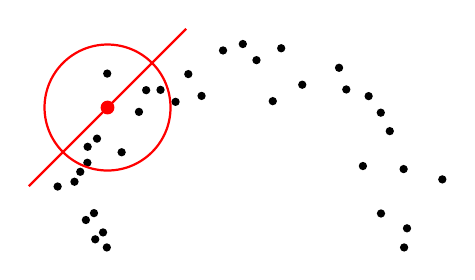
\begin{tikzpicture} 
      \pgfmathsetseed{42}
      % Draw half spiral (from 0 to 180 degrees) with more points
      \foreach \t in {0,5,...,180} {
        \pgfmathsetmacro{\radius}{2.5 - \t/120}
        \pgfmathsetmacro{\noise}{1.0*rnd}
        \pgfmathsetmacro{\x}{(\radius + \noise) * cos(\t)}
        \pgfmathsetmacro{\y}{(\radius + \noise) * sin(\t)}
        
        \fill (\x, \y) circle (1.5pt);
        
        % Store coordinates of 25th point (t=120, since we start at 0 and increment by 5)
        \ifnum\t=120
          \fill[red] (\x, \y) circle (2.5pt);
          \pgfmathsetmacro{\centerx}{\x}
          \pgfmathsetmacro{\centery}{\y}
          \global\let\circlecenterx\centerx
          \global\let\circlecentery\centery
        \fi
      }
      
      % Add red circle centered on the 25th point
      \draw[red, thick] (\circlecenterx, \circlecentery) circle (0.8);
      
      % Add red line cutting through the circle area
      \draw[red, thick] (\circlecenterx - 1, \circlecentery - 1) -- (\circlecenterx + 1, \circlecentery + 1);
    \end{tikzpicture}
    \caption{Local linear embedding assumes that the data is locally linear. } 
    \label{fig:local_linear_embedding}
  \end{figure}

  The concept of neighborhood can be defined in two ways. You can either just fix an $\epsilon$ and take the $\epsilon$-ball around each point $x_i$. Or you can fix a $k$ and take the $k$ nearest neighbors of each point. The general idea of using kernel PCA is to take a local neighborhood of the data and construct some linear approximation of it. 


\section{t-SNE}


\section{UMAP}

  \cite{2018mcinnes}. 


\bibliography{./bibfile}
\bibliographystyle{alpha}
\end{document}
